\documentclass[12pt,a4paper]{article}
\usepackage[utf8]{inputenc}
\usepackage[T1]{fontenc}
\usepackage[brazilian]{babel}
\usepackage{lmodern,microtype,setspace,graphicx,booktabs,tabularx,longtable,array,xcolor,enumitem,fancyhdr,float,listings}
\usepackage[hypcap=false,font=small,labelfont=bf]{caption}
\usepackage[round,authoryear]{natbib}
\usepackage{hyperref}

\usepackage[left=3cm,right=2cm,top=3cm,bottom=2cm]{geometry}
\setstretch{1.5}
\setlength{\parindent}{1.25cm}
\setlength{\parskip}{0pt}
\setlength{\headheight}{15pt}
\emergencystretch=3em
\graphicspath{{../assets/images/}{images/}}

\definecolor{azulufs}{HTML}{174A72}
\definecolor{azulclaro}{HTML}{EAF2F7}
\definecolor{laranja}{HTML}{E84E0F}
\definecolor{verdeclaro}{HTML}{EAF7EF}
\definecolor{verdeforte}{HTML}{147A45}
\definecolor{cinza}{HTML}{F3F5F7}
\definecolor{terminal}{HTML}{0B1220}
\definecolor{terminaltexto}{HTML}{D8E4EC}

\hypersetup{colorlinks=true,linkcolor=azulufs,urlcolor=azulufs,citecolor=azulufs,
  hypertexnames=false,
  pdftitle={Firewall e Roteamento Avancado com OPNsense em Laboratorio Virtual Local},
  pdfauthor={Grupo de Sistemas Operacionais -- UFS}}
\renewcommand{\thesection}{\arabic{section}}
\pagestyle{fancy}\fancyhf{}
\lhead{Firewall e Roteamento Avançado com OPNsense}
\rhead{Sistemas Operacionais}\cfoot{\thepage}
\newcolumntype{Y}{>{\raggedright\arraybackslash}X}
\newcolumntype{P}[1]{>{\raggedright\arraybackslash}p{#1}}
\renewcommand{\arraystretch}{1.2}
\setlist[itemize]{leftmargin=1.1cm,itemsep=2pt,topsep=4pt}
\setlist[enumerate]{leftmargin=1.1cm,itemsep=2pt,topsep=4pt}

\newenvironment{destaque}[1][]{\par\medskip\noindent
 \begin{minipage}{\textwidth}\color{azulufs}\textbf{#1}\par\color{black}}
 {\end{minipage}\par\medskip}
\newenvironment{resultado}[1][]{\par\medskip\noindent
 \begin{minipage}{\textwidth}\color{verdeforte}\textbf{#1}\par\color{black}}
 {\end{minipage}\par\medskip}
\newenvironment{terminalbox}[1][]{\par\medskip\noindent
 \textbf{\texttt{#1}}\par\nobreak}{\par\medskip}
\lstdefinestyle{terminal}{basicstyle=\ttfamily\small\color{terminaltexto},
 backgroundcolor=\color{terminal},breaklines=true,columns=fullflexible,keepspaces=true,
 showstringspaces=false,frame=none}
\lstdefinestyle{codigo}{basicstyle=\ttfamily\small,backgroundcolor=\color{cinza},
 breaklines=true,columns=fullflexible,keepspaces=true,showstringspaces=false,
 frame=single,rulecolor=\color{azulufs!30}}
\newcommand{\arquivo}[1]{\texttt{#1}}
\newcommand{\ip}[1]{\texttt{#1}}

\begin{document}
\pagenumbering{gobble}
\begin{titlepage}
\begin{center}
\textbf{UNIVERSIDADE FEDERAL DE SERGIPE}\\
\textbf{DEPARTAMENTO DE COMPUTAÇÃO}\\
\textbf{DISCIPLINA DE SISTEMAS OPERACIONAIS}
\vspace{1.5cm}

Arthur Felipe Dantas Melo\\Artur Vinícius Santos de Lima\\
Beatriz Baroni Sousa\\Breno Thiago Argemiro Santos\\
Gustavo Gomes Tavares\\Irlan Felipe Alves dos Santos\\
Pedro Guilherme Andrade\\Théo Enderson Conceição de Jesus

\vfill
{\Large\bfseries FIREWALL E ROTEAMENTO AVANÇADO COM OPNSENSE EM LABORATÓRIO VIRTUAL LOCAL\par}
\vfill
São Cristóvão -- SE\\2026
\end{center}
\end{titlepage}

\begin{titlepage}
\begin{center}
Arthur Felipe Dantas Melo; Artur Vinícius Santos de Lima; Beatriz Baroni Sousa;\\
Breno Thiago Argemiro Santos; Gustavo Gomes Tavares; Irlan Felipe Alves dos Santos;\\
Pedro Guilherme Andrade; Théo Enderson Conceição de Jesus
\vfill
{\Large\bfseries FIREWALL E ROTEAMENTO AVANÇADO COM OPNSENSE EM LABORATÓRIO VIRTUAL LOCAL\par}
\vspace{2cm}
\begin{flushright}\begin{minipage}{.54\textwidth}
Trabalho acadêmico apresentado à disciplina de Sistemas Operacionais da
Universidade Federal de Sergipe como documentação do projeto prático de
virtualização, firewall, roteamento, tradução de endereços e rede privada virtual.
\end{minipage}\end{flushright}
\vfill São Cristóvão -- SE\\2026
\end{center}
\end{titlepage}

\pagenumbering{roman}
\section*{Resumo}\addcontentsline{toc}{section}{Resumo}
Este trabalho apresenta a concepção, implementação e validação de um laboratório
virtual local de firewall e roteamento avançado baseado no OPNsense. O ambiente
utiliza KVM/QEMU e libvirt para executar três máquinas virtuais: um firewall,
um cliente interno e um cliente externo. A solução demonstra segmentação entre
LAN e WAN, encaminhamento IP, DNS, tradução de endereços de saída,
redirecionamento de porta, filtragem de tráfego e acesso remoto por WireGuard.
Scripts de instalação, provisionamento e diagnóstico reduzem diferenças entre
distribuições Linux, enquanto um painel web oferece oito ensaios guiados sobre
terminais das máquinas virtuais. Os resultados confirmaram a rota padrão e o NAT, o bloqueio
de conexões não autorizadas, a publicação controlada de um serviço HTTP e o
acesso à LAN pelo túnel VPN. O projeto evidencia como virtualização, isolamento
e automação podem produzir um experimento reproduzível sem infraestrutura de nuvem.

\noindent\textbf{Palavras-chave:} OPNsense. Firewall. Roteamento. NAT. WireGuard. Virtualização.

\newpage
\section*{Abstract}\addcontentsline{toc}{section}{Abstract}
This work presents the design, implementation, and validation of a local virtual
laboratory for advanced firewalling and routing based on OPNsense. KVM/QEMU and
libvirt run three virtual machines: a firewall, an internal client, and an
external client. The solution demonstrates LAN/WAN segmentation, IP forwarding,
DNS, outbound address translation, port forwarding, traffic filtering, and
remote LAN access through WireGuard. Supporting scripts make the environment
reproducible across Linux distributions, while a web dashboard provides eight
guided experiments over the virtual machines' terminals. Results confirmed default routing
and NAT, unauthorized-connection blocking, controlled HTTP publication, and VPN
access to the internal network.

\noindent\textbf{Keywords:} OPNsense. Firewall. Routing. NAT. WireGuard. Virtualization.

\newpage\tableofcontents
\newpage\listoffigures
\newpage\listoftables
\clearpage\pagenumbering{arabic}

\section{Introdução}
Em redes de pequeno porte, decisões sobre endereçamento, rotas, resolução de
nomes e segurança estão diretamente relacionadas. O roteador seleciona o próximo
salto para outras redes, e os serviços de rede tornam esse caminho utilizável
pelas aplicações \citep{kurose2021,tanenbaum2021}. Entretanto, a possibilidade
de encaminhar um pacote não implica que sua passagem deva ser autorizada.

O firewall é o componente responsável por aplicar essa decisão. Segundo o NIST,
ele controla o fluxo de tráfego entre redes ou hosts a partir de uma política de segurança
\citep{nist80041}. Na prática, isso envolve olhar para a interface de entrada,
origem, destino, protocolo, estado da conexão e, quando necessário, tradução de
endereços. O objetivo deste projeto foi tornar essa cadeia de decisões observável
em um laboratório que pudesse ser testado e repetido.

Foi adotado o OPNsense, sistema de firewall e roteamento baseado em FreeBSD,
executado como appliance virtual sobre KVM/QEMU. Duas máquinas Ubuntu compõem os
extremos interno e externo da topologia. A execução local assegura que as redes,
as máquinas virtuais e as políticas possam ser observadas e reproduzidas no
próprio ambiente de estudo, sem dependência de infraestrutura externa.

\subsection{Problema e motivação}
Em uma aula prática, é comum enxergar uma regra de firewall em uma tela, executar
um \texttt{ping} em outra e tratar a VPN como uma terceira atividade. O problema
é que o caminho entre esses pontos fica escondido. Além disso, um laboratório
montado apenas por passos manuais costuma quebrar quando muda a distribuição
Linux, a permissão do usuário ou a versão do hipervisor.

O laboratório integra essas partes em uma única sequência de observação. Cada
regra é relacionada à topologia, à finalidade de segurança e a um teste
observável. O painel web apresenta os comandos e a saída devolvida pelas máquinas
virtuais, de modo que a interface visual não substitui a evidência técnica, mas
a torna mais fácil de interpretar.

\subsection{Objetivos}
O objetivo geral é implementar e documentar um laboratório virtual local de
firewall e roteamento avançado. São objetivos específicos:
\begin{itemize}
\item segmentar LAN, WAN simulada e rede WireGuard;
\item configurar gateway, DNS, NAT de saída e filtragem com estado;
\item publicar seletivamente um serviço por DNAT, mantendo os demais acessos bloqueados;
\item permitir acesso autenticado à LAN por WireGuard;
\item automatizar instalação, importação, provisionamento e diagnóstico em Linux;
\item validar cada propriedade por comandos reais e critérios reproduzíveis.
\end{itemize}

\section{Fundamentação teórica}
\subsection{FreeBSD e OPNsense}
O FreeBSD é um sistema operacional do tipo Unix cujo manual abrange administração
de rede, segurança, firewalls e virtualização \citep{freebsdhandbook}. O OPNsense
utiliza essa base em uma distribuição especializada, com interface web,
filtragem por estado, NAT, serviços de rede e VPN \citep{opnsensedocs}. No
laboratório, todas as rotas entre domínios passam pelo firewall, onde podem ser
autorizadas, traduzidas ou rejeitadas.

\subsection{Endereçamento, roteamento e gateway}
Os blocos privados definidos pela RFC 1918 podem ser utilizados internamente sem
coordenação com registros globais, mas não devem ser propagados na Internet
pública \citep{rfc1918}. Empregam-se \ip{192.168.10.0/24} para a LAN e
\ip{10.10.10.0/24} para a WAN simulada. A separação obriga o tráfego entre
clientes a passar pelo OPNsense.

Quando o destino não pertence à rede diretamente conectada, a estação entrega o
pacote ao gateway padrão, que consulta sua tabela de roteamento
\citep{kurose2021,tanenbaum2021}. No cliente LAN, a rota aponta para
\ip{192.168.10.1}, endereço interno do OPNsense. Essa propriedade é validada
antes dos testes externos.

Essa relação entre cliente, gateway e rede externa é apresentada visualmente na
Figura~\ref{fig:gateway}. No cenário implementado, o OPNsense ocupa a posição
central: ele recebe os pacotes que deixam a LAN, consulta suas rotas e aplica a
política de saída antes de encaminhá-los para a WAN.

\begin{figure}[H]\centering
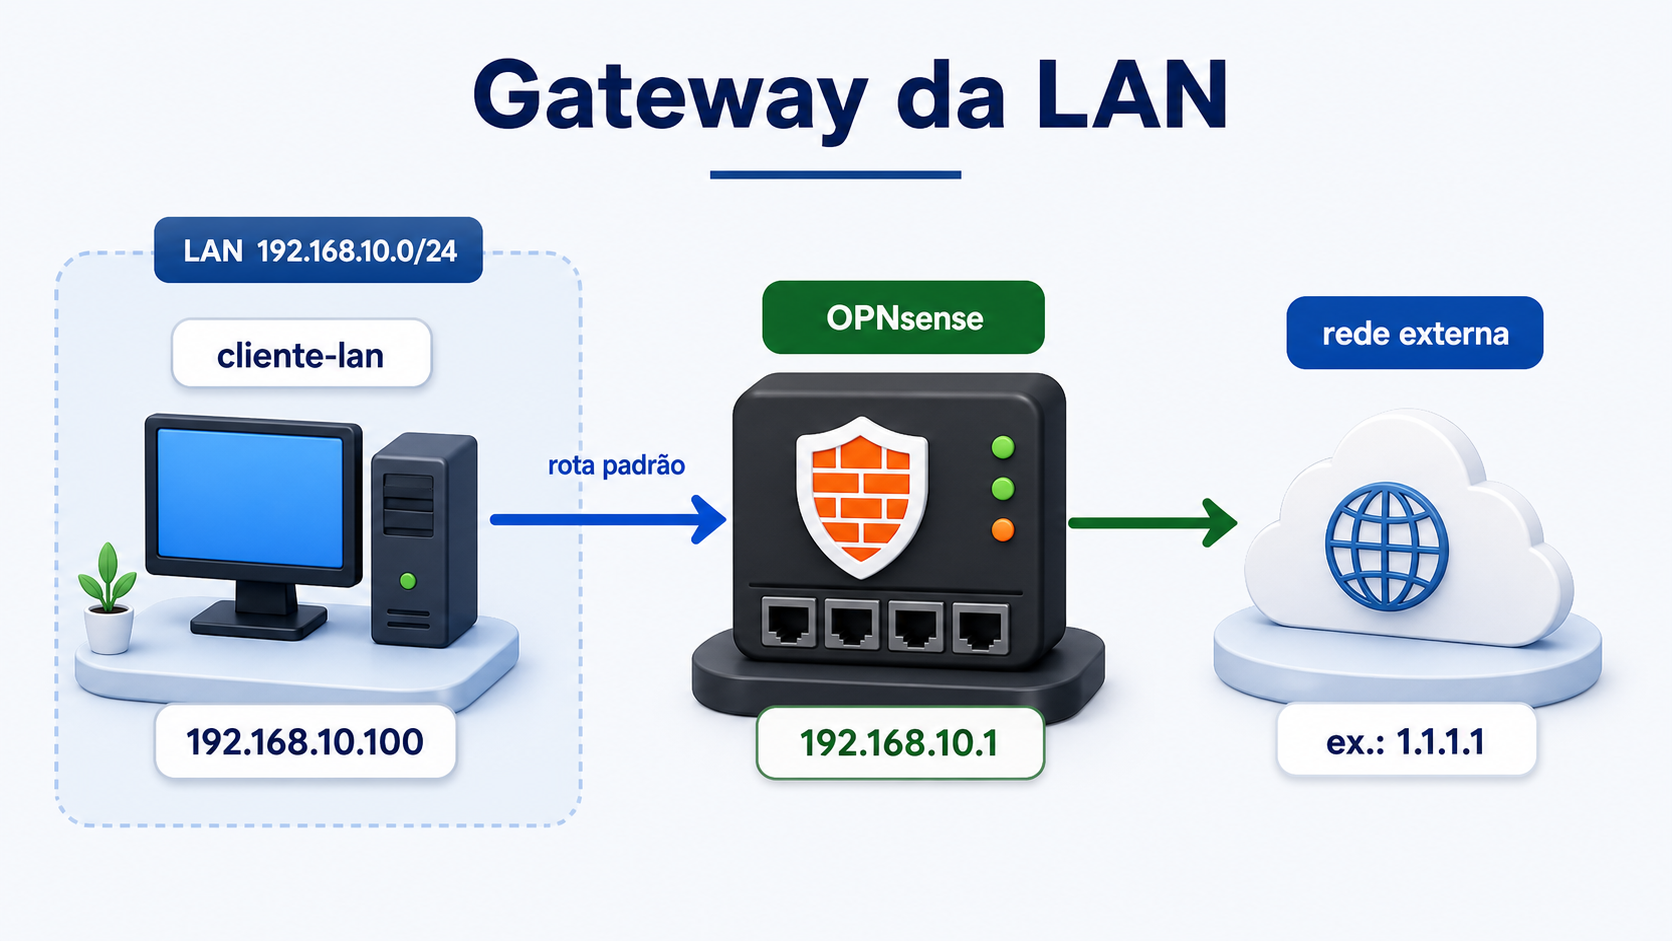
\includegraphics[width=.94\textwidth]{gateway-lan-visual.png}
\caption{OPNsense como gateway padrão da LAN. \textit{Fonte: elaboração do grupo (2026).}}
\label{fig:gateway}
\end{figure}

\subsection{DHCP e DNS}
O DHCP fornece parâmetros de configuração por uma troca cliente-servidor,
incluindo endereço, máscara, roteador e servidores de nomes \citep{rfc2131}.
Para que o destino do DNAT permaneça determinístico, o cliente de demonstração
utiliza \ip{192.168.10.100} estático; em produção, uma reserva DHCP atenderia ao
mesmo requisito com administração centralizada.

O DNS define um espaço hierárquico de nomes e operações de consulta distribuída
\citep{rfc1035}. A resolução externa é testada separadamente da conectividade
por IP: alcançar \ip{1.1.1.1} evidencia rota e retorno, enquanto resolver
\texttt{one.one.one.one} acrescenta evidência do caminho DNS.

A Figura~\ref{fig:dhcpdns} separa as duas responsabilidades: DHCP entrega os
parâmetros de rede e DNS transforma um nome em endereço IP. A ilustração
representa o comportamento do serviço de LAN. Para manter a regra de DNAT
reprodutível, o cliente usado na demonstração final recebe os mesmos parâmetros
por configuração estática; gateway e DNS continuam apontando para o OPNsense.

\begin{figure}[H]\centering
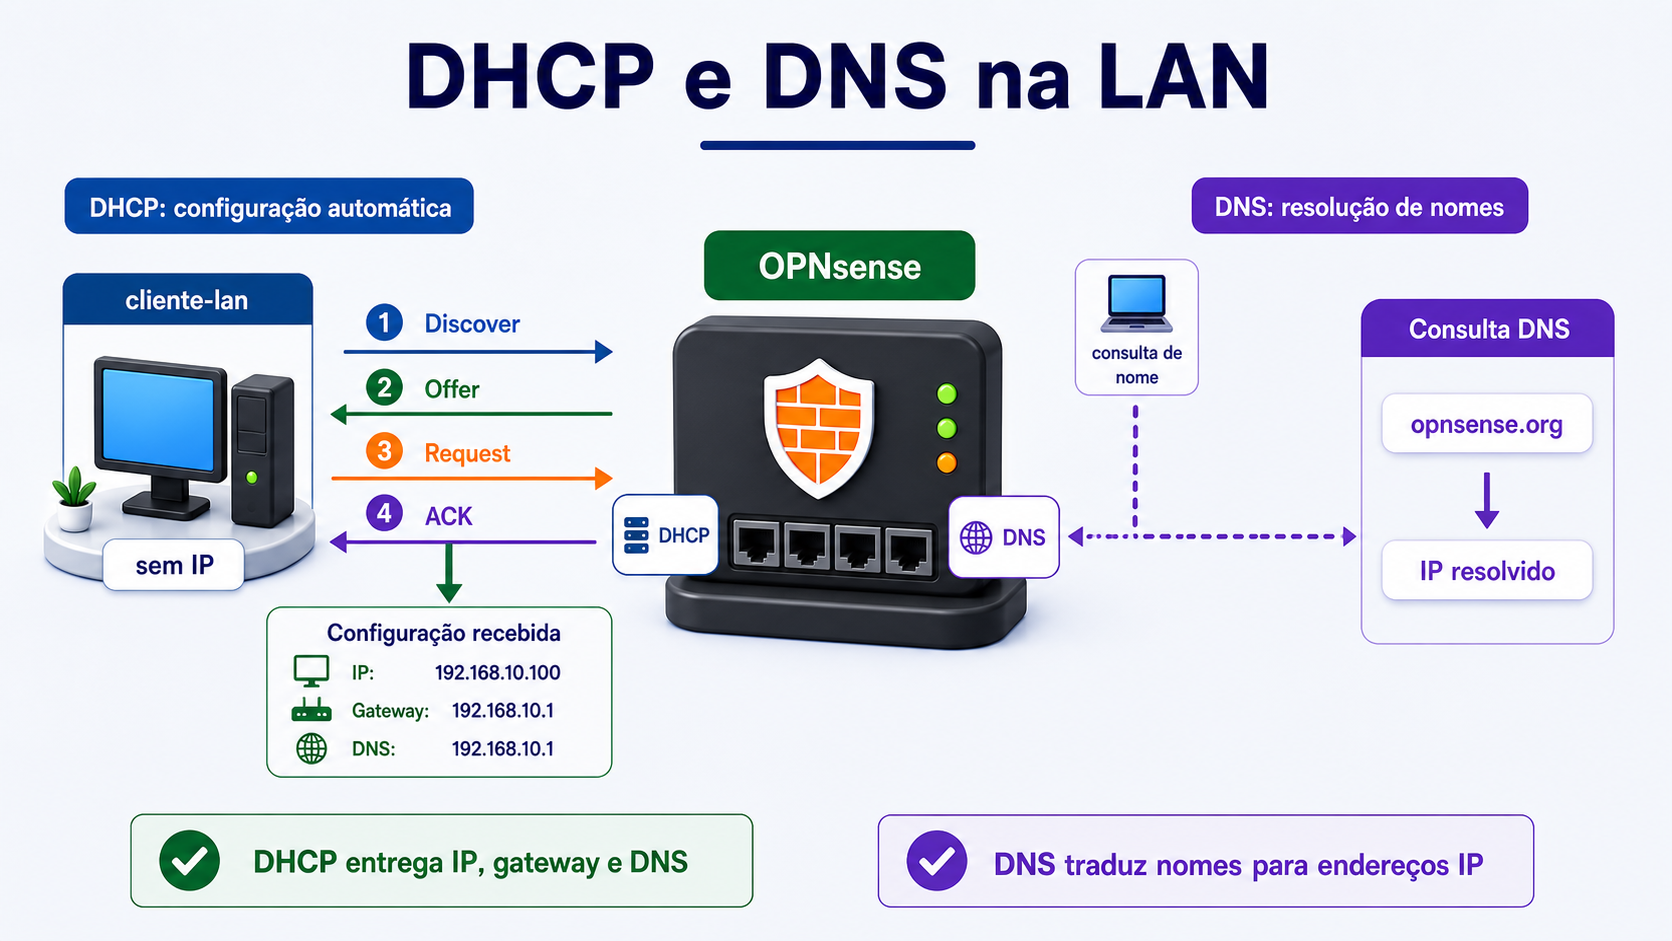
\includegraphics[width=.94\textwidth]{dhcp-dns-lan-visual.png}
\caption{Serviços DHCP e DNS disponibilizados à LAN. \textit{Fonte: elaboração do grupo (2026).}}
\label{fig:dhcpdns}
\end{figure}

\subsection{NAT e DNAT}
O NAT mapeia endereços de um domínio para outro. Na modalidade NAPT, sessões
também são diferenciadas por portas TCP ou UDP \citep{rfc3022}. Na saída, o
OPNsense substitui a origem privada e mantém estado para devolver as respostas.
No DNAT, conexões destinadas ao firewall são reescritas para um servidor
interno. A regra demonstrada recebe TCP em \ip{10.10.10.146:8080} e encaminha
para \ip{192.168.10.100:8080}; isso não abre a LAN, pois apenas o fluxo descrito
é autorizado.

\subsection{Firewall com estado}
A política de firewall especifica o tráfego permitido e o tratamento do restante.
O NIST recomenda regras baseadas em requisitos e revisadas sistematicamente
\citep{nist80041}. Firewalls com estado acompanham conexões e distinguem o
retorno de uma sessão autorizada de uma nova tentativa externa
\citep{cheswick2003}. O experimento adota exposição mínima: LAN inicia conexões;
WAN não acessa diretamente a LAN; DNAT e VPN são exceções explícitas.

\subsection{WireGuard}
O WireGuard associa peers a chaves públicas e conjuntos de endereços permitidos.
Seu desenho busca uma base pequena, criptografia moderna e uma interface de
configuração semelhante à de um dispositivo de rede \citep{donenfeld2017}. O
cliente WAN usa \ip{10.99.0.2}; o OPNsense usa \ip{10.99.0.1} e UDP
\ip{51820}. A validação observa handshake e alcance da ponta VPN, do gateway e
do cliente LAN, distinguindo uma interface ativa de um túnel funcional.

\subsection{Virtualização}
Virtualização executa sistemas convidados sobre recursos físicos compartilhados,
com fronteiras de administração e isolamento. Redes virtuais, hipervisor e
convidados passam a compor a superfície administrada \citep{nist800125}. KVM
fornece virtualização no kernel Linux, QEMU modela máquina e dispositivos, e
libvirt gerencia domínios, redes e volumes. As redes \texttt{lan-lab} e
\texttt{wan-lab} substituem switches físicos sem alterar a rede real do local.

\section{Metodologia}
O trabalho tem caráter aplicado e experimental. Foram definidos requisitos de
rede e segurança: a LAN deveria sair pela rota padrão, a WAN não poderia entrar
livremente, o HTTP só apareceria pela regra de DNAT e a VPN teria de chegar à
rede interna. A partir desses requisitos, a topologia foi construída e cada
propriedade recebeu um ensaio próprio. Um \textit{timeout}, por exemplo, não é
tratado como erro por padrão; no teste de bloqueio, ele é justamente a evidência
esperada.

Para favorecer a repetição do experimento, a configuração foi organizada em
scripts de instalação, criação de redes, importação de máquinas e
provisionamento. Essa separação reduz a interferência de particularidades do
host no resultado do estudo e permite concentrar a análise nos protocolos, nas
regras e nos fluxos de tráfego.

\subsection{Componentes}
\begin{table}[H]\centering
\caption{Componentes do laboratório.}\label{tab:componentes}
\begin{tabularx}{\textwidth}{P{3cm}YY}\toprule
\textbf{Componente}&\textbf{Função}&\textbf{Justificativa}\\\midrule
OPNsense&Firewall, roteador, NAT, DNS e VPN&Centraliza a política e a inspeção.\\
KVM/QEMU&Execução das VMs&Integração ao kernel e desempenho próximo ao nativo.\\
libvirt&Redes, volumes e domínios&Automação por \texttt{virsh} e XML.\\
Ubuntu Server&Clientes LAN e WAN&Ambiente enxuto com ferramentas de rede.\\
Aplicação web&Dashboard e terminal&Apresentação guiada das evidências produzidas pelas VMs.\\
Cockpit&Administração visual&Confirma estado e console dos convidados.\\\bottomrule
\end{tabularx}\end{table}

\subsection{Topologia e endereçamento}
A topologia parte de três convidados: o \texttt{cliente-lan}, o
\texttt{cliente-wan} e o \texttt{opnsense-fw}. O firewall fica entre os dois
clientes e participa das três redes do experimento: WAN, LAN e WireGuard. É ele
quem concentra gateway, DNS, NAT, DNAT e a política de filtragem. A Figura
\ref{fig:topologia-visual} apresenta essa relação de forma mais direta.

O desenho original ainda registra a etapa em que o laboratório podia ser
administrado remotamente. Na versão entregue, porém, KVM/libvirt, Cockpit e o
dashboard são executados no computador do participante. A topologia de rede não
mudou; apenas a administração ficou local e independente de infraestrutura externa.

\begin{figure}[H]\centering
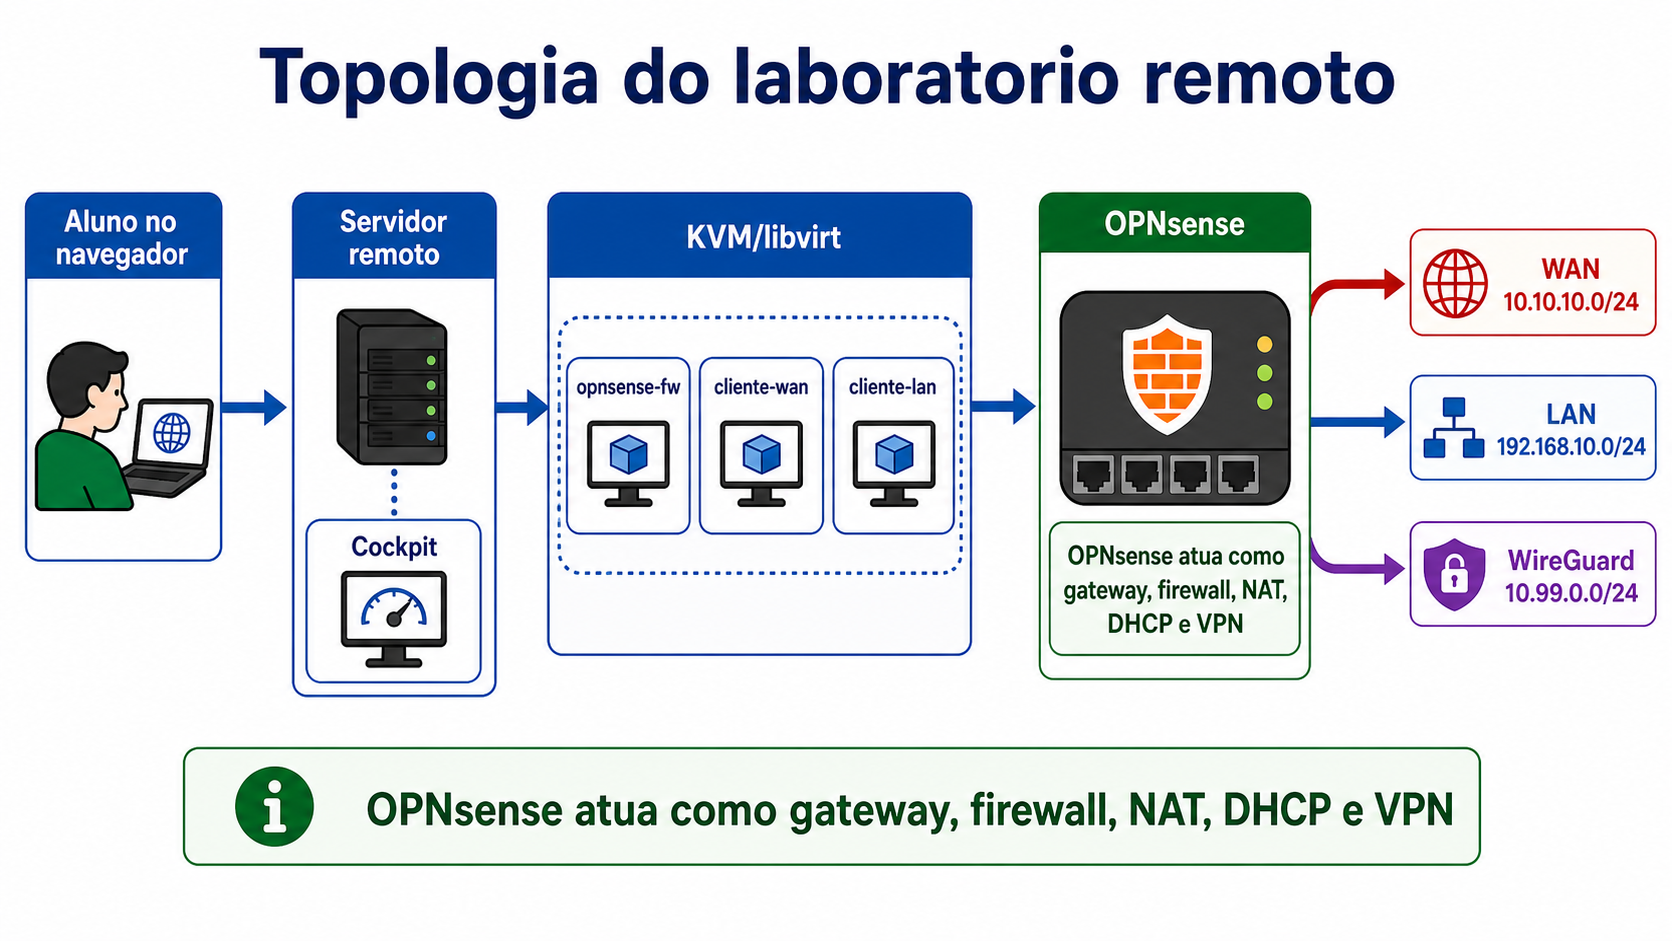
\includegraphics[width=\textwidth]{topologia-laboratorio-completa.png}
\caption{Visão arquitetural do laboratório: convidados, OPNsense e redes WAN, LAN e WireGuard. \textit{Fonte: elaboração do grupo (2026).}}
\label{fig:topologia-visual}
\end{figure}

\begin{table}[H]\centering
\caption{Plano de endereçamento.}\label{tab:enderecos}
\begin{tabularx}{\textwidth}{P{3cm}P{4cm}Y}\toprule
\textbf{Domínio}&\textbf{Endereço}&\textbf{Papel}\\\midrule
WAN&\ip{10.10.10.0/24}&Segmento externo simulado.\\
OPNsense WAN&\ip{10.10.10.146/24}&Entrada externa, DNAT e VPN.\\
Cliente WAN&\ip{10.10.10.171/24}&Origem dos testes externos.\\
LAN&\ip{192.168.10.0/24}&Segmento interno protegido.\\
OPNsense LAN&\ip{192.168.10.1/24}&Gateway e referência DNS.\\
Cliente LAN&\ip{192.168.10.100/24}&Estação e servidor HTTP.\\
WireGuard&\ip{10.99.0.0/24}&Túnel entre WAN e firewall.\\\bottomrule
\end{tabularx}\end{table}

\subsection{Implantação}
A implantação foi organizada como uma sequência controlada: preparação do host,
definição das redes virtuais, importação das máquinas, configuração dos clientes
e disponibilização das interfaces de acompanhamento. O procedimento completo e
os requisitos de cada sistema operacional permanecem documentados no repositório,
pois constituem material operacional de apoio, e não o foco analítico deste
trabalho.

Essa organização separa dois níveis do projeto. O primeiro é o objeto de estudo:
endereçamento, roteamento, NAT, filtragem e VPN. O segundo é a infraestrutura
necessária para reproduzi-lo. Manter essa distinção evita que detalhes de
instalação desviem a discussão dos princípios de rede que o laboratório pretende
demonstrar.

\section{Implementação}
\subsection{Estrutura do repositório}
\begin{lstlisting}[style=codigo,caption={Estrutura resumida do projeto.}]
.
|-- app/              # dashboard FastAPI
|-- assets/           # imagens da entrega
|-- docs/             # topologia e diagnostico
|-- infra/            # instalacao e provisionamento
|   |-- lib/common.sh
|   `-- vm-config/    # redes e dominios libvirt
|-- paper/            # relatorio LaTeX
|-- presentation/     # apresentacao em PDF
|-- local/            # VMs e chaves; ignorado pelo Git
`-- docker-compose.yml
\end{lstlisting}
O repositório separa o código do dashboard, as definições de infraestrutura, os
materiais visuais e a documentação. Essa organização não é apenas administrativa:
ela torna explícita a relação entre a configuração que produz o ambiente e as
evidências usadas para analisá-lo.

\subsection{Reprodutibilidade do ambiente}
A execução local foi escolhida para que o cenário possa ser reconstruído sem
depender de serviços de terceiros. As imagens das máquinas, as definições de rede
e os procedimentos de configuração são mantidos separados dos artefatos de
apresentação e do texto acadêmico. Com isso, o leitor pode distinguir aquilo que
é resultado do experimento daquilo que é apenas suporte para sua reprodução.

Em termos pedagógicos, essa decisão é relevante porque permite repetir os testes,
alterar uma regra e comparar o novo comportamento com a evidência anterior. O
laboratório, portanto, não é apresentado como uma configuração estática, mas
como um espaço controlado para observar as consequências de decisões de rede.

\subsection{Política de tráfego}
\begin{table}[H]\centering
\caption{Síntese da política validada.}\label{tab:politica}
\begin{tabularx}{\textwidth}{P{2.4cm}P{3cm}P{2.6cm}Y}\toprule
\textbf{Origem}&\textbf{Destino}&\textbf{Ação}&\textbf{Finalidade}\\\midrule
LAN&WAN/Internet&Permitir com NAT&Saída e resolução externa.\\
WAN&LAN direta&Bloquear&Impedir acesso iniciado externamente.\\
WAN TCP 8080&LAN:8080&Permitir com DNAT&Publicar somente o HTTP.\\
WAN UDP 51820&OPNsense&Permitir&Estabelecer WireGuard.\\
WireGuard&LAN&Permitir&Acesso autenticado à rede protegida.\\\bottomrule
\end{tabularx}\end{table}

As cinco figuras seguintes sintetizam a política em ordem de leitura. Primeiro,
a LAN é autorizada a iniciar conexões para fora; depois, a WAN é impedida de
iniciar sessões diretamente contra o cliente interno. As três regras seguintes
introduzem somente as exceções necessárias: publicação HTTP por DNAT, chegada do
túnel WireGuard ao firewall e acesso do peer autenticado à LAN. Essa sequência é
importante porque mostra que o projeto não se resume a permitir tráfego: ele
define quais caminhos existem e em quais condições.

\begin{figure}[H]\centering
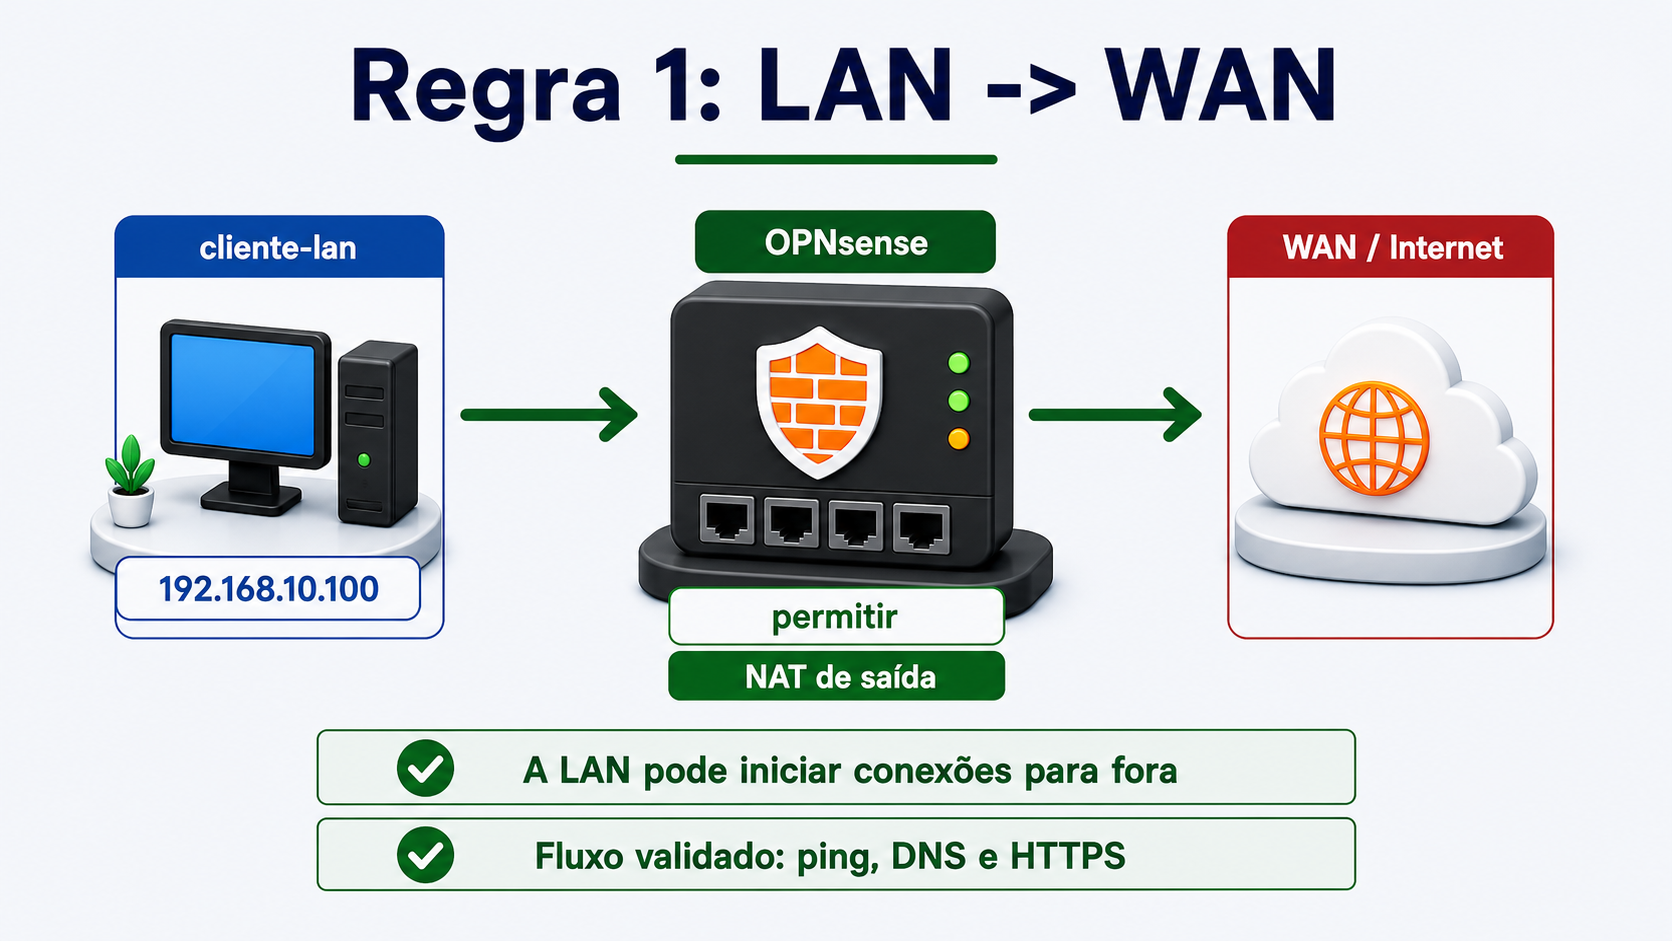
\includegraphics[width=.94\textwidth]{firewall-regra-01-lan-wan.png}
\caption{Regra 1: a LAN inicia conexões para a WAN com NAT de saída. \textit{Fonte: elaboração do grupo (2026).}}
\label{fig:regra-lan-wan}
\end{figure}

O fluxo da Figura~\ref{fig:regra-lan-wan} é validado pela rota padrão do cliente
LAN e pelo retorno de pacotes ICMP. A permissão é iniciada internamente; o
firewall com estado admite as respostas correspondentes, sem converter isso em
uma abertura geral da WAN para a LAN.

\begin{figure}[H]\centering
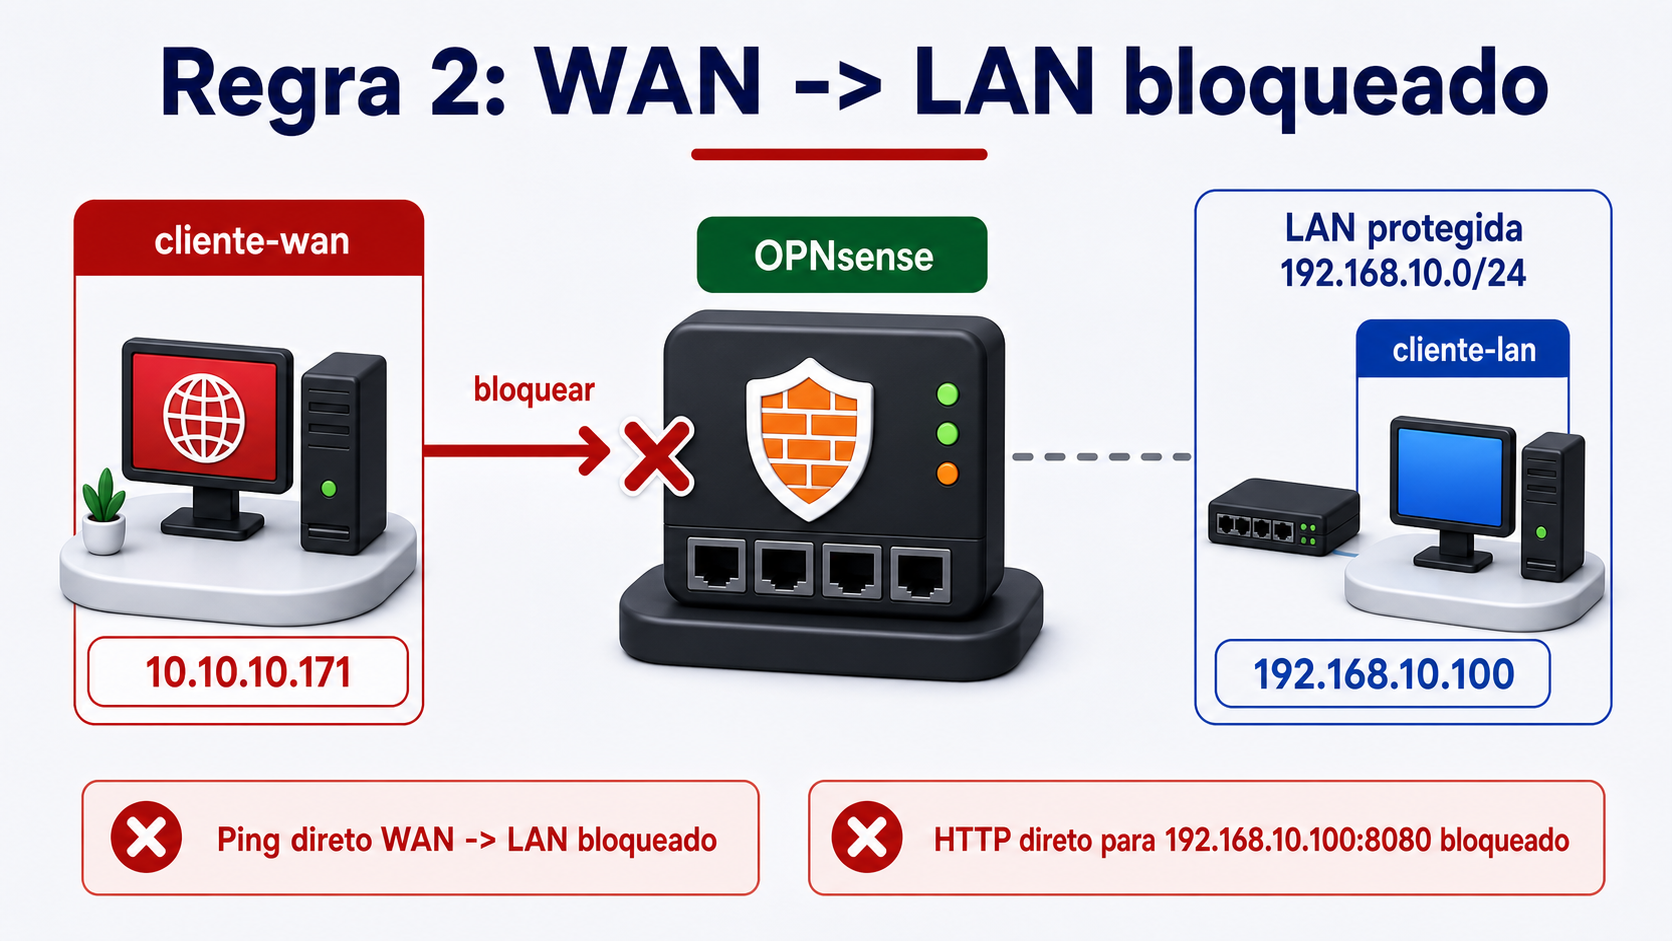
\includegraphics[width=.94\textwidth]{firewall-regra-02-wan-lan-bloqueado.png}
\caption{Regra 2: conexões diretas da WAN para a LAN permanecem bloqueadas. \textit{Fonte: elaboração do grupo (2026).}}
\label{fig:regra-wan-bloqueada}
\end{figure}

A Figura~\ref{fig:regra-wan-bloqueada} corresponde ao teste negativo do roteiro:
o cliente externo não obtém resposta por ICMP nem abre conexão HTTP diretamente
para \ip{192.168.10.100:8080}. Essa ausência de resposta é evidência da política
de isolamento, e não uma falha do experimento.

\begin{figure}[H]\centering
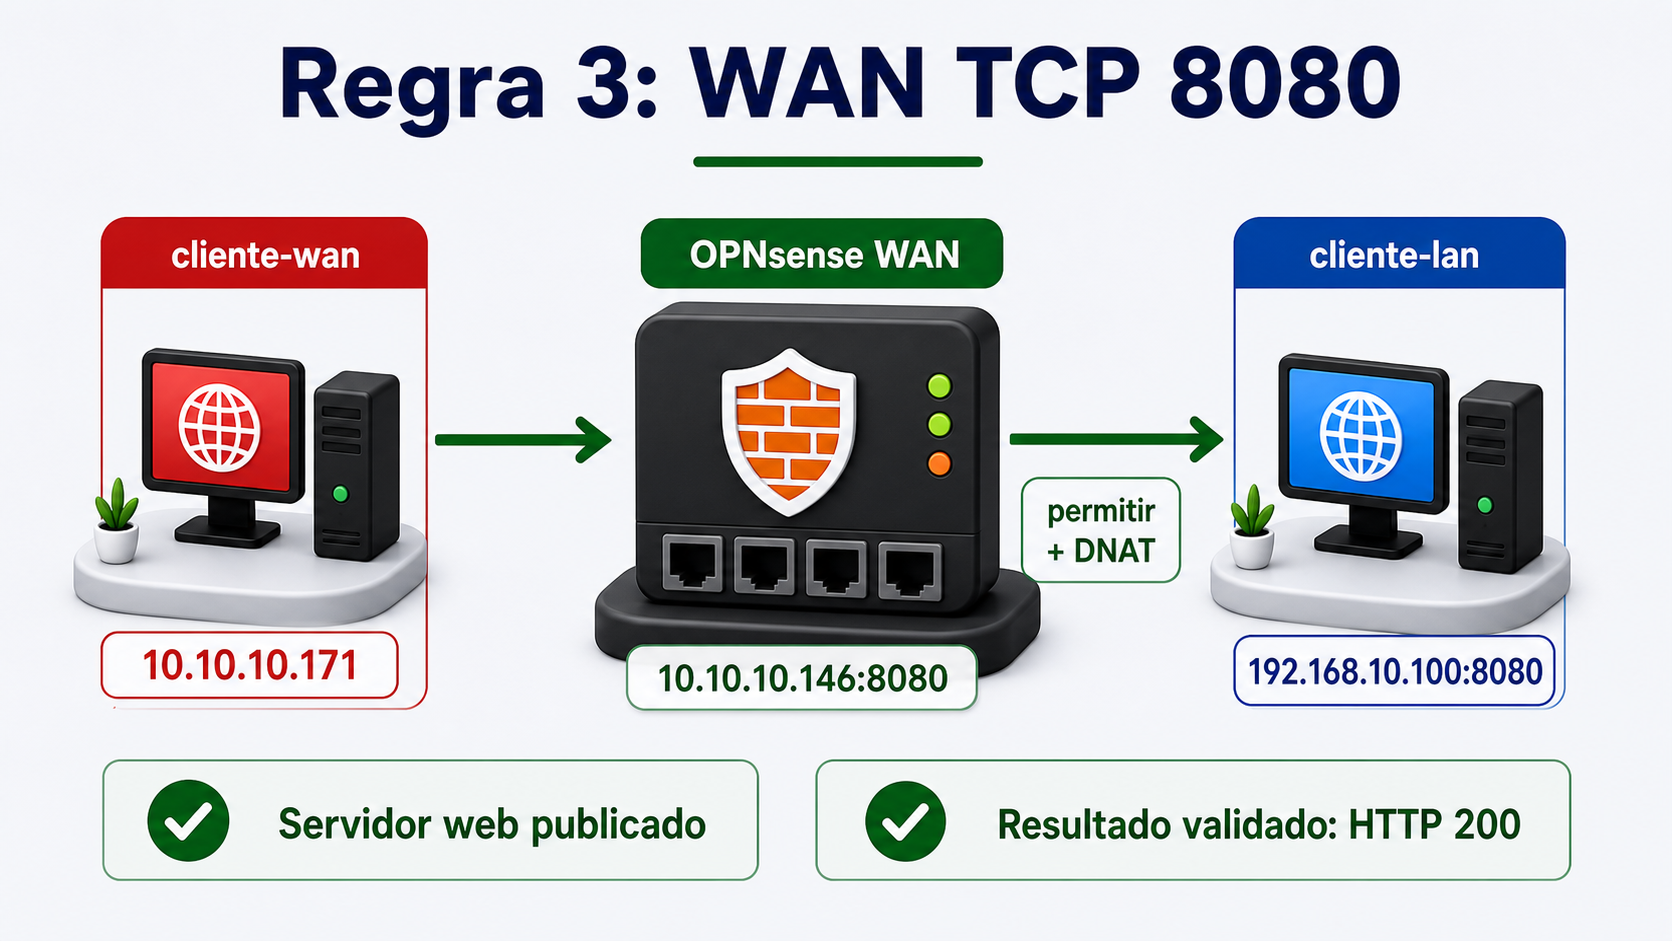
\includegraphics[width=.94\textwidth]{firewall-regra-03-wan-tcp-8080-dnat.png}
\caption{Regra 3: publicação HTTP por DNAT na porta TCP 8080. \textit{Fonte: elaboração do grupo (2026).}}\label{fig:dnat}
\end{figure}

A publicação mostrada na Figura~\ref{fig:dnat} é a exceção controlada à regra
anterior. O acesso é feito ao endereço WAN do OPNsense, não diretamente ao
cliente LAN; apenas TCP na porta \ip{8080} é traduzido para o serviço temporário.

\begin{figure}[H]\centering
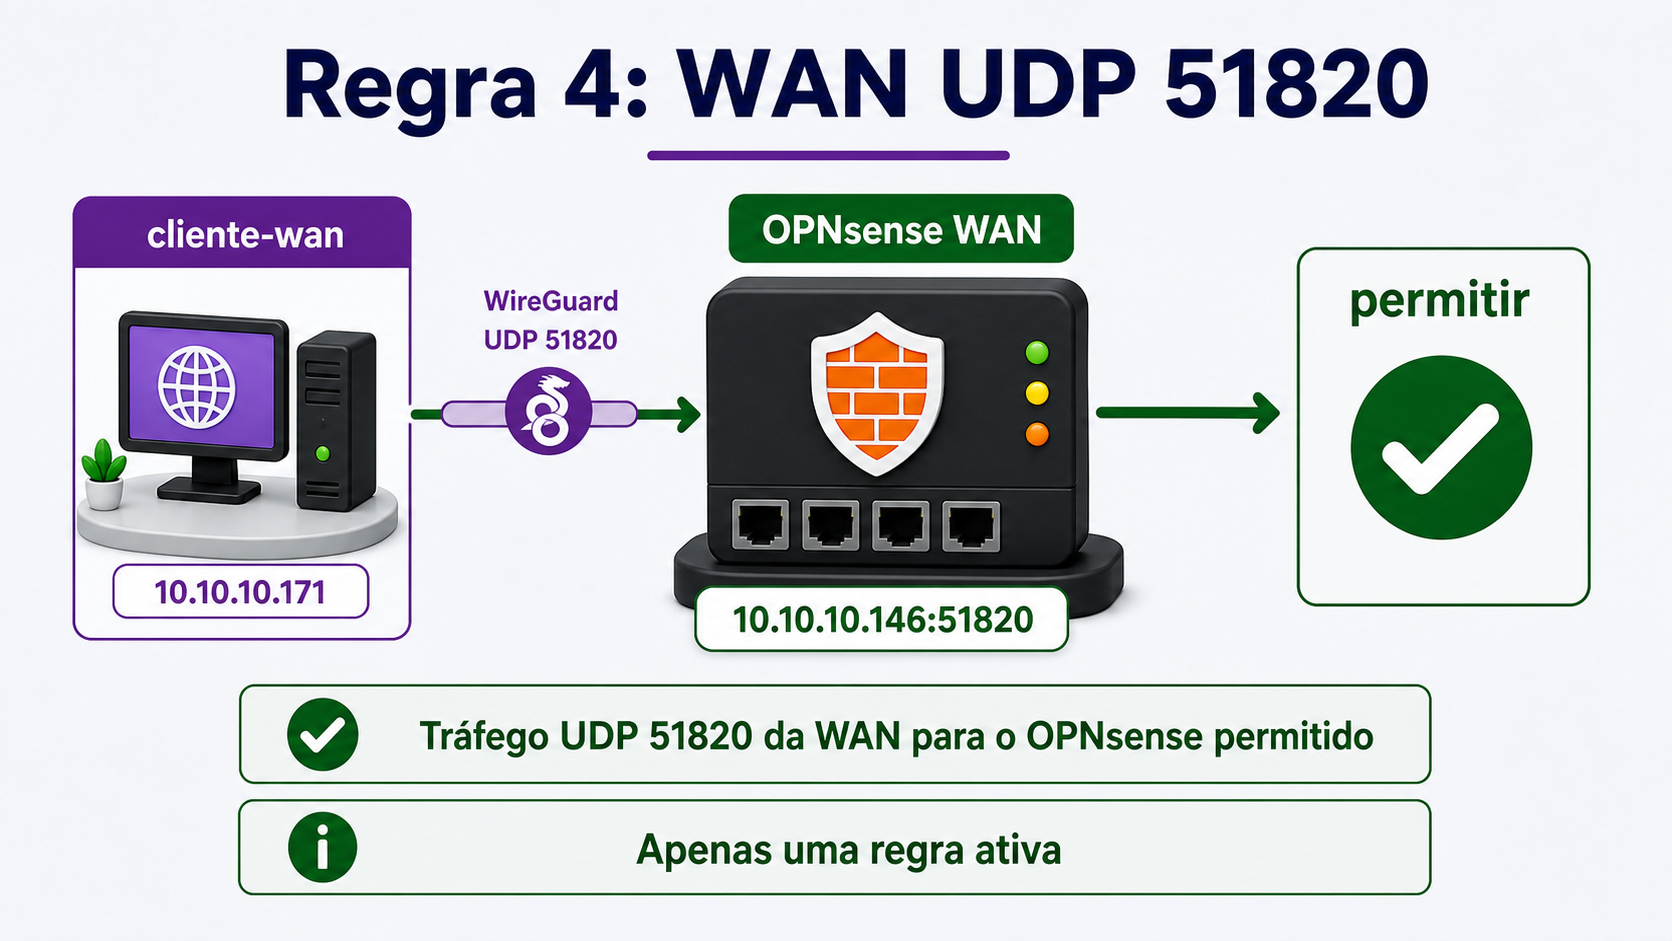
\includegraphics[width=.94\textwidth]{firewall-regra-04-wan-udp-51820-wireguard.png}
\caption{Regra 4: tráfego UDP 51820 permitido para o endpoint WireGuard. \textit{Fonte: elaboração do grupo (2026).}}\label{fig:regra-wg-udp}
\end{figure}

A Figura~\ref{fig:regra-wg-udp} mostra que o firewall aceita UDP \ip{51820}
somente para o endpoint VPN. A autorização dessa porta cria o caminho do túnel,
mas ainda não concede, por si só, acesso irrestrito à LAN.

\begin{figure}[H]\centering
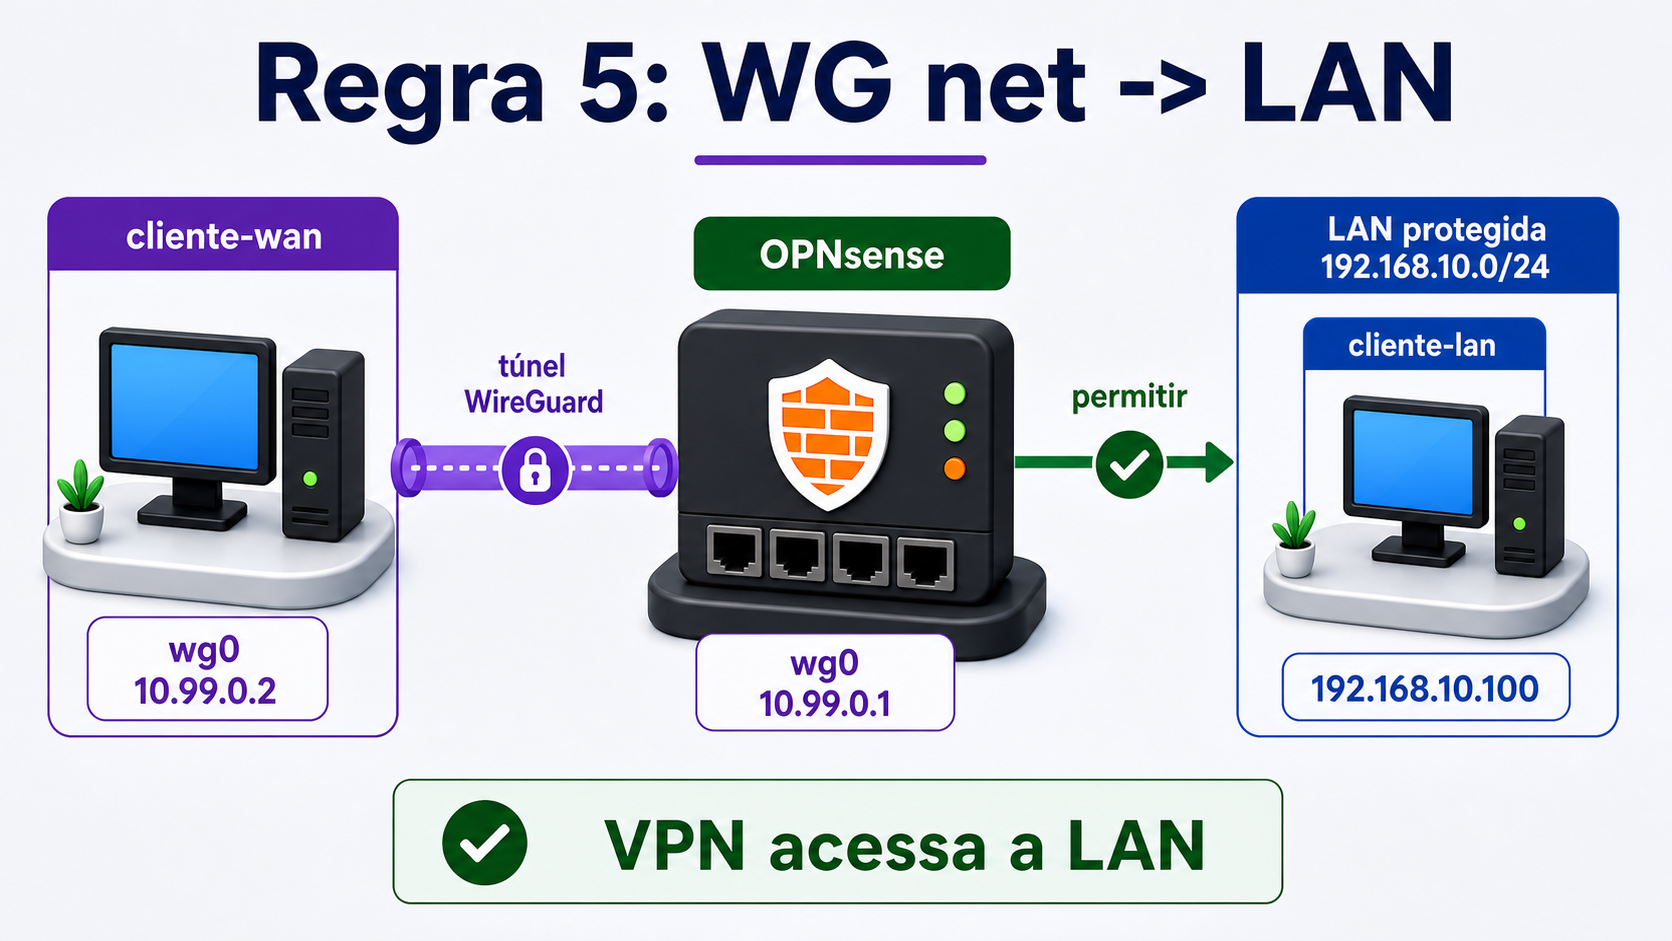
\includegraphics[width=.94\textwidth]{firewall-regra-05-wg-net-lan.png}
\caption{Regra 5: peer WireGuard autorizado a alcançar a LAN. \textit{Fonte: elaboração do grupo (2026).}}\label{fig:wg}
\end{figure}

Somente após o handshake e a regra representada na Figura~\ref{fig:wg}, o peer
\ip{10.99.0.2} alcança o gateway \ip{192.168.10.1} e o cliente
\ip{192.168.10.100}. O último ensaio do dashboard verifica exatamente essa
progressão, tornando visível a diferença entre abrir a porta de VPN e autorizar
o tráfego de VPN para a rede protegida.

\subsection{Dashboard de validação}
O painel de validação fica disponível em \url{http://localhost:8088}. Ele organiza
os oito testes em uma sequência coerente: primeiro a
configuração básica, depois saída, bloqueio, DNAT e VPN. Em cada cartão há o
comando que pode ser copiado, o que se espera observar e um terminal da máquina
envolvida. Dessa forma, quem acompanha consegue entender a intenção antes de
olhar para a saída.

O terminal apresentado no painel está conectado às máquinas virtuais. Assim,
prompt, comando, cores e mensagens correspondem à sessão efetivamente executada
no convidado. O botão \textit{Executar} envia os mesmos comandos exibidos na
tela, um por vez. Os testes de conectividade também possuem limite de tempo,
para que uma conexão bloqueada seja registrada como evidência sem interromper a
sequência de validação.

\IfFileExists{images/dashboard-local.png}{
\begin{figure}[H]\centering
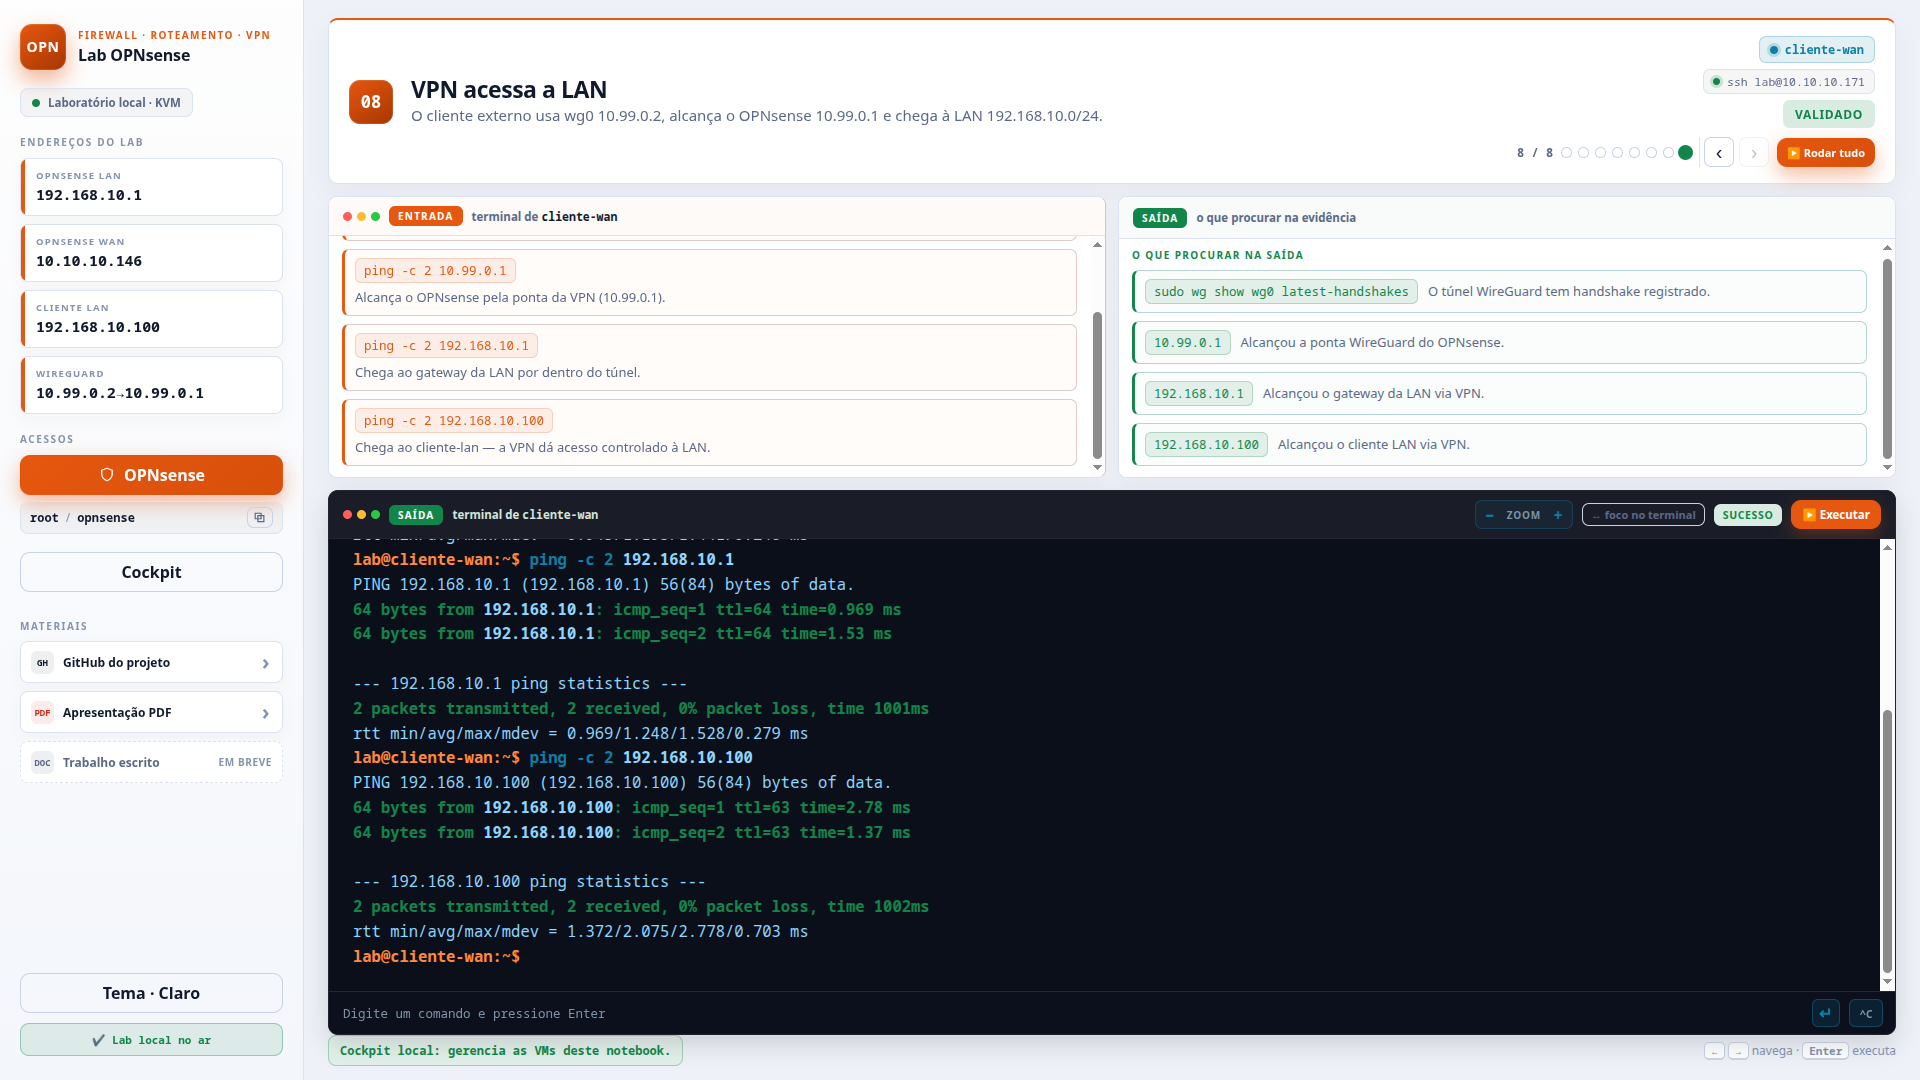
\includegraphics[width=\textwidth]{images/dashboard-local.png}
\caption{Painel de validação durante o ensaio de acesso à LAN por WireGuard. \textit{Fonte: captura dos autores (2026).}}\label{fig:dashboard}
\end{figure}}{}

\subsection{Interfaces de operação e observabilidade}
Além do dashboard, o ambiente mantém dois pontos de administração. O primeiro é
o painel do OPNsense, usado para acompanhar interfaces, gateways, serviços e o
estado do WireGuard. O segundo é o Cockpit, exposto somente no host local, que
permite consultar e operar as VMs pelo navegador. As capturas seguintes foram
realizadas no laboratório em execução e registram essas duas camadas de operação.

\IfFileExists{images/opnsense-dashboard.png}{
\begin{figure}[H]\centering
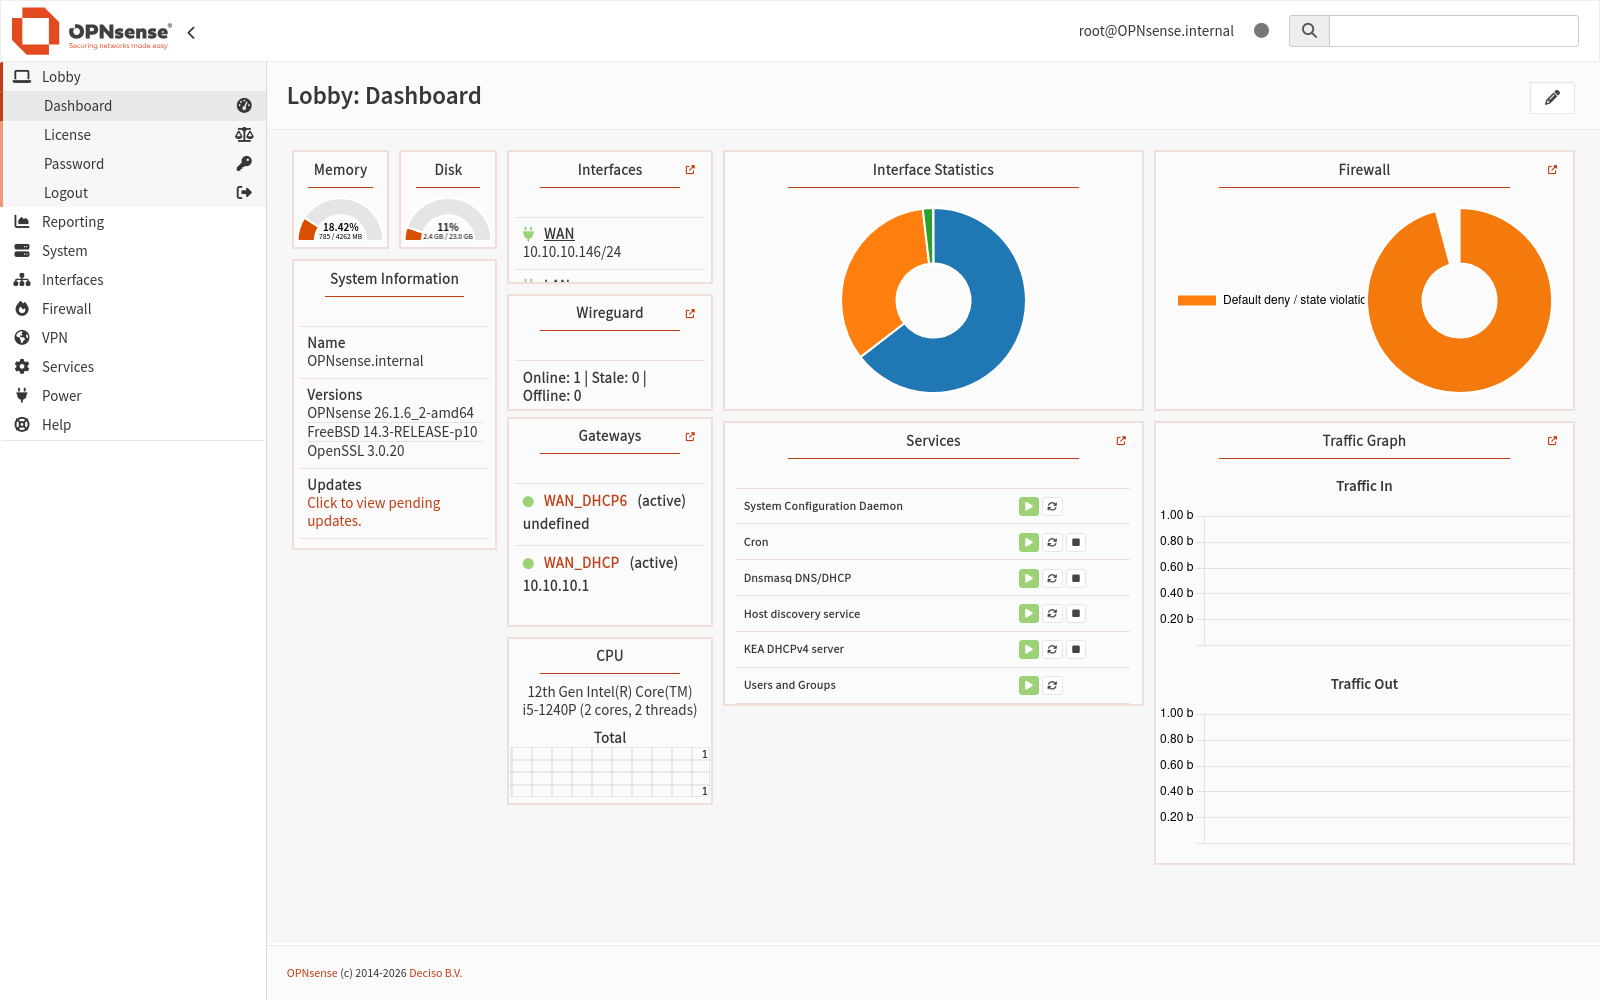
\includegraphics[width=\textwidth]{images/opnsense-dashboard.png}
\caption{Painel administrativo do OPNsense em execução: interfaces, WireGuard, gateways e serviços. \textit{Fonte: captura dos autores (2026).}}\label{fig:opnsense-dashboard}
\end{figure}}{}

\IfFileExists{images/cockpit-local.png}{
\begin{figure}[H]\centering
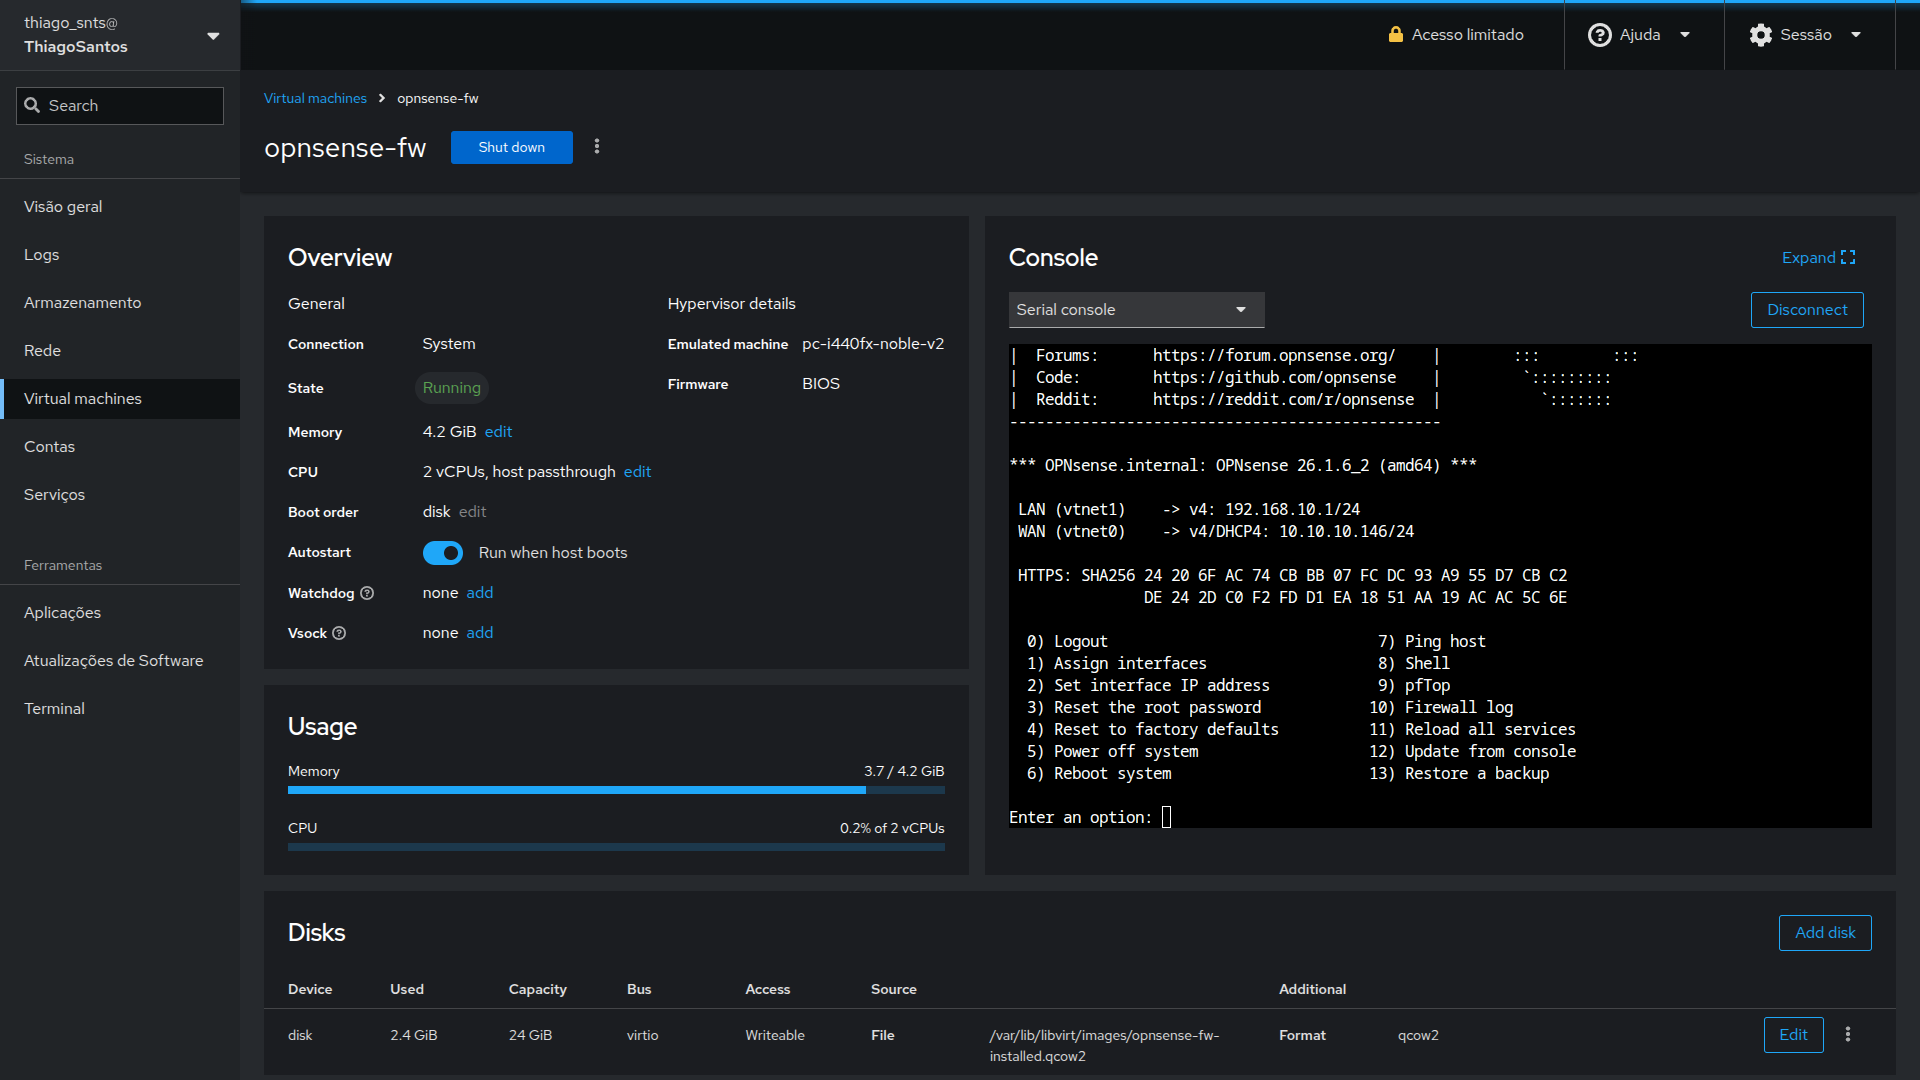
\includegraphics[width=\textwidth]{images/cockpit-local.png}
\caption{Cockpit em execução, com a VM OPNsense selecionada e seu console serial disponível para observação. \textit{Fonte: captura dos autores (2026).}}\label{fig:cockpit}
\end{figure}}{}

\section{Validação e resultados}
Os ensaios foram ordenados para reduzir dependências ocultas: configuração local,
saída externa, serviço controlado, isolamento da WAN, DNAT, limpeza e VPN.
\begin{longtable}{P{.6cm}P{3.1cm}P{5.1cm}P{4.5cm}}
\caption{Resultados dos oito ensaios.}\label{tab:resultados}\\\toprule
\textbf{N.}&\textbf{Propriedade}&\textbf{Critério}&\textbf{Resultado}\\\midrule\endfirsthead
\toprule\textbf{N.}&\textbf{Propriedade}&\textbf{Critério}&\textbf{Resultado}\\\midrule\endhead
1&Endereço e rota&\ip{192.168.10.100/24}; rota via \ip{192.168.10.1}.&Correspondentes; aprovado.\\
2&DNS&DNS \ip{192.168.10.1} e resolução externa.&Nome resolvido; aprovado.\\
3&Rota/NAT&Rota para \ip{1.1.1.1} via OPNsense; 0\% de perda.&Duas respostas; aprovado.\\
4&Servidor HTTP&Socket em \ip{0.0.0.0:8080}.&\texttt{LISTEN}; aprovado.\\
5&Bloqueio WAN&Ping à LAN sem resposta; porta WAN 80 expira.&100\% de perda e timeout; aprovado.\\
6&DNAT&Acesso à WAN:8080 retorna conteúdo do servidor LAN.&HTTP recebido; aprovado.\\
7&Encerramento&Processo finalizado e porta liberada.&Porta 8080 liberada; aprovado.\\
8&WireGuard&Handshake e alcance de WG, gateway e cliente LAN.&Três destinos responderam; aprovado.\\\bottomrule
\end{longtable}

\subsection{Evidências representativas}
\begin{terminalbox}[Rota padrão e NAT]
\begin{lstlisting}[style=terminal]
lab@cliente-lan:~$ ip route get 1.1.1.1
1.1.1.1 via 192.168.10.1 dev enp1s0 src 192.168.10.100 uid 1000
lab@cliente-lan:~$ ping -c 2 1.1.1.1
64 bytes from 1.1.1.1: icmp_seq=1 ttl=62 time=28.1 ms
64 bytes from 1.1.1.1: icmp_seq=2 ttl=62 time=28.2 ms
2 packets transmitted, 2 received, 0% packet loss
\end{lstlisting}\end{terminalbox}

O teste de bloqueio é um resultado negativo esperado. A ausência de resposta é
comparada à política: como o cliente WAN está operacional, mas não abre sessão
direta na LAN, o timeout evidencia a restrição.
\begin{terminalbox}[Bloqueio direto da WAN]
\begin{lstlisting}[style=terminal]
lab@cliente-wan:~$ ping -c 2 -W 2 192.168.10.100
2 packets transmitted, 0 received, 100% packet loss
lab@cliente-wan:~$ curl --connect-timeout 3 --max-time 5 http://10.10.10.146:80/
curl: (28) Failed to connect: Timeout was reached
\end{lstlisting}\end{terminalbox}

Na etapa seguinte, o mesmo cliente acessa a porta publicada. O contraste mostra
que a permissão é seletiva, não consequência de roteamento irrestrito.
\begin{terminalbox}[Publicação por DNAT]
\begin{lstlisting}[style=terminal]
lab@cliente-wan:~$ curl --connect-timeout 3 --max-time 5 http://10.10.10.146:8080/
<!DOCTYPE HTML>
<html lang="en"> ... </html>
\end{lstlisting}\end{terminalbox}

\begin{terminalbox}[WireGuard de ponta a ponta]
\begin{lstlisting}[style=terminal]
lab@cliente-wan:~$ sudo wg show wg0 latest-handshakes
22+X5bXkPk3LnQT4K5PznNGbTvid3NAU7wi4op8D9zc= <timestamp>
lab@cliente-wan:~$ ping -c 2 10.99.0.1
2 packets transmitted, 2 received, 0% packet loss
lab@cliente-wan:~$ ping -c 2 192.168.10.1
2 packets transmitted, 2 received, 0% packet loss
lab@cliente-wan:~$ ping -c 2 192.168.10.100
2 packets transmitted, 2 received, 0% packet loss
\end{lstlisting}\end{terminalbox}

Os oito ensaios foram aprovados em mais de um host Linux. O conjunto comprova
mais que a simples execução das VMs: relaciona configuração, encaminhamento,
isolamento, exceção controlada e VPN em uma cadeia de evidências coerente.
\begin{resultado}[Síntese]
O laboratório confirmou, por comandos nos convidados, segmentação LAN/WAN,
rota pelo OPNsense, NAT, bloqueio externo, DNAT TCP 8080 e acesso WireGuard à LAN.
\end{resultado}

\section{Alternativas e decisões de projeto}
\subsection{OPNsense e pfSense}
Ambos são alternativas baseadas em FreeBSD com firewall, NAT e VPN. O OPNsense
foi mantido por compor o escopo, possuir documentação oficial e integrar as
funções usadas \citep{opnsensedocs}. Isso não implica superioridade universal:
uma equipe com processos consolidados no pfSense poderia reduzir custos mantendo-o.

\subsection{KVM/libvirt e VirtualBox}
VirtualBox possui interface conhecida e suporte a vários hosts. KVM/libvirt se
integra ao kernel Linux, oferece automação por \texttt{virsh} e redes declarativas.
Como o público executa Linux, KVM reduz camadas. O trade-off é uma instalação
mais sensível a grupos, serviço libvirt e virtualização na BIOS/UEFI.

\subsection{WireGuard, OpenVPN e IPsec}
OpenVPN oferece ampla compatibilidade e material acumulado; IPsec é padronizado
e comum entre equipamentos. WireGuard foi escolhido pelo modelo compacto de
peers, configuração pequena e criptografia moderna \citep{donenfeld2017}.
Autenticação corporativa ou interoperabilidade legada poderiam favorecer as
alternativas.

\subsection{IP estático e reserva DHCP}
DHCP é adequado a estações comuns \citep{rfc2131}, mas o DNAT exige destino
estável. Adotou-se \ip{192.168.10.100} estático para tornar a imagem e o teste
determinísticos. Em produção, reserva DHCP combinaria estabilidade e gestão
central, evitando o risco de duplicidade da configuração manual.

\subsection{Dashboard e ferramentas nativas}
Cockpit, console libvirt e acesso por terminal seriam suficientes para operar o
ambiente. O dashboard acrescenta uma camada didática: ordena as verificações,
explicita os critérios e aproxima cada comando do conceito que ele evidencia.
Como mantém a possibilidade de entrada manual e apresenta a saída das VMs, a
interface organiza a observação sem ocultar o funcionamento do sistema.

\section{Reprodutibilidade, limitações e segurança}
O repositório reúne as definições de infraestrutura, a aplicação de
acompanhamento e a documentação necessária para reconstruir o experimento.
Imagens de máquinas virtuais são distribuídas separadamente por seu tamanho e
por representarem o estado do ambiente. Essa divisão preserva o versionamento do
material acadêmico sem comprometer a possibilidade de reprodução.

O cenário não mede vazão, latência sob carga ou resistência a ataques. A WAN é
simulada e compartilha hardware pelo hipervisor, apesar do isolamento lógico.
DNS e Internet dependem da rede do host. Os oito testes verificam requisitos
selecionados, mas não substituem revisão integral de regras, análise de logs e
testes de intrusão autorizados \citep{nist80041}.

O dashboard deve permanecer restrito ao host local, pois expõe recursos de
operação das VMs. Em qualquer implantação que ultrapasse o escopo didático,
credenciais administrativas, exposição de serviços e regras de DNAT devem ser
tratadas segundo princípios de menor privilégio e administração contínua.

\section{Conclusão}
O projeto integrou sistemas operacionais, virtualização e redes em um único
experimento. KVM/QEMU e libvirt forneceram o isolamento necessário à topologia;
o OPNsense concentrou encaminhamento, filtragem, NAT e VPN; e os clientes
produziram evidências para cada política analisada. A automação foi utilizada
como meio de reprodução, permitindo que a atenção permaneça nos fenômenos de
rede observados.

Os resultados mostraram que a LAN utiliza o OPNsense como gateway e alcança
destinos externos por NAT; que a WAN não acessa diretamente a LAN; que um serviço
é publicado seletivamente por DNAT; e que um peer WireGuard alcança a rede
protegida. A repetição em hosts Linux distintos reforça a reprodutibilidade.

Como continuidade, podem-se incorporar coleta de logs, medição de desempenho
entre VPNs, regressão automática das regras e reservas DHCP. Essas extensões
permitiriam avaliar desempenho, observabilidade e evolução da política.

\newpage\renewcommand{\refname}{Referências}
\addcontentsline{toc}{section}{Referências}
\begin{thebibliography}{99}
\bibitem[Cheswick, Bellovin e Rubin(2003)]{cheswick2003}
CHESWICK, W. R.; BELLOVIN, S. M.; RUBIN, A. D. \textbf{Firewalls and Internet Security: Repelling the Wily Hacker}. 2. ed. Boston: Addison-Wesley, 2003.
\bibitem[Donenfeld(2017)]{donenfeld2017}
DONENFELD, J. A. WireGuard: Next Generation Kernel Network Tunnel. In: \textbf{Network and Distributed System Security Symposium}. San Diego: Internet Society, 2017. DOI: \url{https://doi.org/10.14722/ndss.2017.23160}.
\bibitem[Droms(1997)]{rfc2131}
DROMS, R. \textbf{Dynamic Host Configuration Protocol}. RFC 2131. IETF, 1997. Disponível em: \url{https://www.rfc-editor.org/rfc/rfc2131}.
\bibitem[FreeBSD Documentation Project(2026)]{freebsdhandbook}
FREEBSD DOCUMENTATION PROJECT. \textbf{FreeBSD Handbook}. Disponível em: \url{https://docs.freebsd.org/en/books/handbook/}.
\bibitem[Kurose e Ross(2021)]{kurose2021}
KUROSE, J. F.; ROSS, K. W. \textbf{Redes de computadores e a Internet: uma abordagem top-down}. 8. ed. São Paulo: Pearson, 2021.
\bibitem[Mockapetris(1987)]{rfc1035}
MOCKAPETRIS, P. \textbf{Domain Names: Implementation and Specification}. RFC 1035. IETF, 1987. Disponível em: \url{https://www.rfc-editor.org/rfc/rfc1035}.
\bibitem[OPNsense Project(2026)]{opnsensedocs}
OPNSENSE PROJECT. \textbf{OPNsense Documentation}. Disponível em: \url{https://docs.opnsense.org/}.
\bibitem[Rekhter et al.(1996)]{rfc1918}
REKHTER, Y. et al. \textbf{Address Allocation for Private Internets}. RFC 1918. IETF, 1996. DOI: \url{https://doi.org/10.17487/RFC1918}.
\bibitem[Scarfone e Hoffman(2009)]{nist80041}
SCARFONE, K.; HOFFMAN, P. \textbf{Guidelines on Firewalls and Firewall Policy}. NIST SP 800-41 Rev. 1. Gaithersburg: NIST, 2009. DOI: \url{https://doi.org/10.6028/NIST.SP.800-41r1}.
\bibitem[Scarfone, Souppaya e Hoffman(2011)]{nist800125}
SCARFONE, K.; SOUPPAYA, M.; HOFFMAN, P. \textbf{Guide to Security for Full Virtualization Technologies}. NIST SP 800-125. Gaithersburg: NIST, 2011. DOI: \url{https://doi.org/10.6028/NIST.SP.800-125}.
\bibitem[Srisuresh e Egevang(2001)]{rfc3022}
SRISURESH, P.; EGEVANG, K. \textbf{Traditional IP Network Address Translator (Traditional NAT)}. RFC 3022. IETF, 2001. DOI: \url{https://doi.org/10.17487/RFC3022}.
\bibitem[Tanenbaum, Feamster e Wetherall(2021)]{tanenbaum2021}
TANENBAUM, A. S.; FEAMSTER, N.; WETHERALL, D. \textbf{Redes de computadores}. 6. ed. Porto Alegre: Bookman, 2021.
\end{thebibliography}

\appendix\newpage
\section{Roteiro mínimo de reprodução}
\begin{enumerate}
\item Clonar o repositório e instalar dependências. Em seguida, executar:
\begin{lstlisting}[style=codigo]
sudo bash infra/install-prereqs.sh
\end{lstlisting}
\item Consultar \arquivo{INSTALACAO.md} para os requisitos e os arquivos de máquina virtual.
\item Executar o roteiro de preparação indicado em \arquivo{COMO\_RODAR.md}.
\item Abrir \url{http://localhost:8088} e realizar os oito ensaios propostos.
\item Usar o Cockpit ou a interface do OPNsense para complementar a observação do ambiente.
\end{enumerate}

\section{Matriz de rastreabilidade}
\begin{table}[H]\centering
\caption{Relação entre objetivo, implementação e evidência.}
\begin{tabularx}{\textwidth}{P{3.2cm}YY}\toprule
\textbf{Objetivo}&\textbf{Implementação}&\textbf{Evidência}\\\midrule
Segmentar redes&Redes libvirt e OPNsense com duas interfaces&Endereços distintos e bloqueio WAN--LAN.\\
Prover saída da LAN&Rota e NAT no OPNsense&Ensaio 3, gateway e 0\% de perda.\\
Publicar serviço&DNAT TCP 8080&Ensaios 4 a 7.\\
Acesso seguro&WireGuard e regra WG--LAN&Ensaio 8, handshake e três destinos.\\
Reproduzir o estudo&Materiais de instalação e configuração&Execução em diferentes hosts Linux.\\\bottomrule
\end{tabularx}\end{table}
\end{document}
